\chapter{Introduction}
\label{chap:introduction}

\section{Standard Model}
Everything in the universe is found to be made up of a few basic building blocks called fundamental particles, governed by four fundamental forces. The four forces (electromagnetic, weak, strong, and gravity) are categorized by their force carriers and strength. The Standard Model of particle physics is a theory concerning the electromagnetic, weak, and strong nuclear interactions, as well as classifying all the subatomic particles known. It has successfully explained almost all experimental results and provided a variety of precise experimental predictions. According to the Standard Model, the fundamental particles are divided into two basic types called quarks and leptons. Each group consists of six particles, and all of them are with spin = 1/2 known as fermions. The three fundamental forces included in Standard Model result from the exchange of force-carrier particles. The gluon mediates the strong force which is described by quantum chromodynamics (QCD). The electromagnetic force is mediated by photon and initially described by quantum electrodynamics (QED). The weak force is mediated by W$^{\pm}$ and Z bosons. The electromagnetic force and weak force were unified. The Higgs boson explaining why the other elementary particles (except the photon and gluon) are massive, was tentatively confirmed to exist on 14 March 2013. Figure~\ref{standardModel} shows the fundamental particles and force carriers.

\begin{figure}[htbp]
\centering
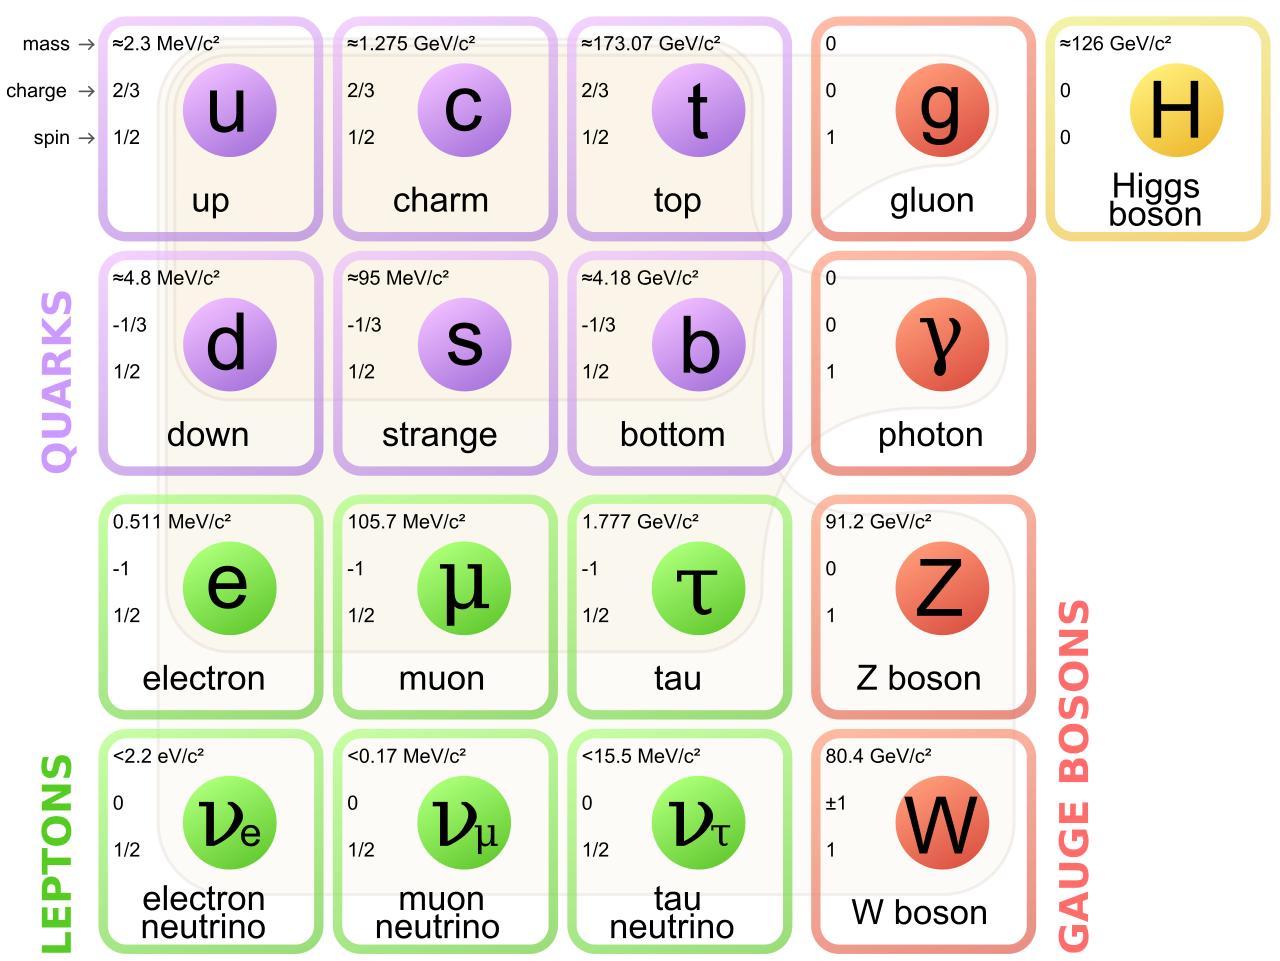
\includegraphics[keepaspectratio,width=0.8\textwidth]{introduction/Standard_Model.png}
\figcaption{The Standard Model of elementary particles and force carriers. This picture is from Wikipedia.}
 \label{standardModel}
\end{figure}

\section{Quantum Chromodynamics}
Quantum Chromodynamics (QCD) is a renormalized non-abelian gauge theory based on the $SU(3)_{C}$ group~\cite{QCDtheory} to describe strong interactions between quarks and gluons. The subscript $C$ denotes the quantum number - color, which is an exact symmetry. Quarks are color triplets while hadrons are assumed to be color singlets in QCD. The invariant QCD Lagrangian requires gauge (gluon) self-interactions due to the non-abelian character of the $SU(3)_{C}$ group. There are eight different gluons, and the gluon exchange can change the color of a quark but not its flavor. QCD has two seemingly-contradictory properties: 1) Asymptotic freedom; 2) Confinement.

\subsection{Asymptotic Freedom and Confinement}
Experimentally, no single quark has ever been isolated. Only the color-neutral quark bound states - hadrons ($q\bar{q}$, $qqq$ or $\bar{q}\bar{q}\bar{q}$) can be observed. This suggests the interaction between quarks and gluons must be strong on large distance scale. However, in the deep inelastic scattering experiments. It was found that with large momentum transfer, the quarks inside the hadron behaved as if they were almost free~\cite{DISasymptotic}. According to the behaviors of short and long distance, the static QCD potential can be described as:
\begin{equation} 
V_{s} = -\frac{4}{3} \times \frac{\alpha_{s}}{r} + k \times r 
\label{QCDpotential}
\end{equation}
where the first term dominating at small distance is similar to the Coulomb potential between two charges in QED, while the second term is linked to the confinement of quarks and gluons inside hadrons.  

The effect coupling constant depends on the renormalization scale, which can be written as: 
\begin{equation} 
\alpha_{s}(\mu) = \frac{g^{2}_{s}(\mu)}{4\pi} \approx \frac{4\pi}{\beta_{0}ln(\mu^{2}/\Lambda^{2}_{QCD})} 
\label{runningConst}
\end{equation}
where $\beta_{0} = (11 - \frac{2}{3}n_{f})$ is a constant, depending on the number of active quark flavors at the energy scale $\mu$ and $\Lambda_{QCD}$ is a constant QCD scale parameter determined experimentally ($\Lambda_{QCD}\approx$ 250 MeV/$c$). Figure~\ref{runningConstant} shows the experimental measurements of $\alpha_{s}$ as a function of Q (momentum transfer)~\cite{runningExp}.

\begin{figure}[htbp]
\centering
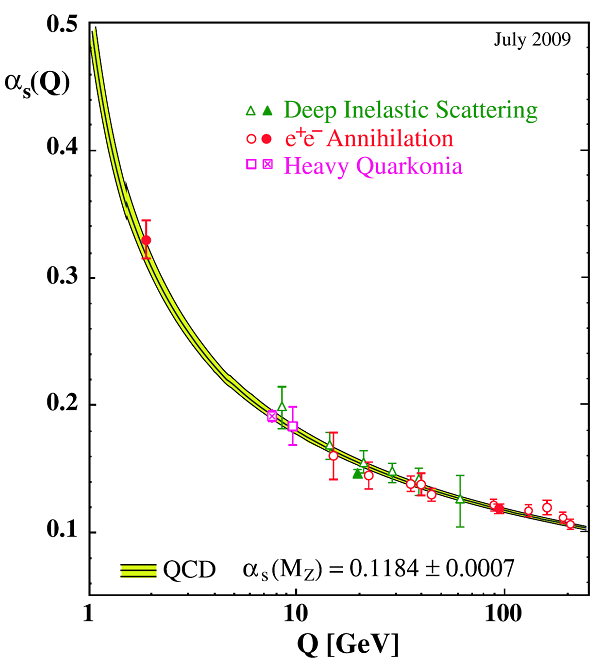
\includegraphics[keepaspectratio,width=0.7\textwidth]{introduction/running_constant.png}
\figcaption{Experimentally measured $\alpha_{s}$ as function of the respective
energy scale Q~\cite{runningExp}.}
 \label{runningConstant}
\end{figure}

With larger $Q^{2}$ (probing small length scales), the $\alpha_{s}$ becomes smaller. The small $\alpha_{s}$ suggests that the quarks and gluons move freely. When $\alpha_{s}\ll$ 1 (high momentum transfer or short distance approach), methods of perturbative QCD (pQCD) are applied to predict the cross sections and distributions of physical processes implying quarks and gluons in the initial, intermediate or final state. On the contrary, with smaller $Q^{2}$ or larger distance ($\alpha_{s}\rightarrow$ 1), the attractive force and gluon binding potential between quarks become larger. When quarks separate, the gluon field form narrow tubes (or strings) of color charge to bring the quarks together. When two quarks have large enough energies and become separated, at some point the gluon field is more energetically favorable to create a new quark and anti-quark pair out of the vacuum than to allow the quarks to separate further. As a result, a new hadron is created instead of seeing free quarks. The QCD coupling constant $\alpha_{s}$ approaches unity quickly as momentum transfer decreases in low-momentum transfer processes. In this case, the high order processes will have large contributions and can not be neglected, thus the pQCD is not valid any more. Instead, the Lattice QCD or other Non-Perturbative QCD (e.g. AdS/CTF - anti-de-Sitter space/conformal field theory) is used to calculate strong interaction processes.

\subsection{Quark Gluon Plasma and Phase Transition}
Quark Matter is mostly observed as quark bound state in normal condition. However, in extreme condition like high temperature or high baryon density, quarks and gluons are proposed to be deconfined from a hadron. A new state of deconfined matter is thus created, so called Quark Gluon Plasma (QGP). In such an environment, long-range interactions are screened by the high density of color charges. Since short-range interactions in QCD are weak, the quarks and gluons (partons) behave as nearly free particles. Lattice QCD calculations show that significant change of $\varepsilon/T^{4}$ ($\varepsilon$ - energy density, $T$ - temperature, this quantity is proportional to the number of degrees of freedom) occurs at the critical temperature ($T_{c}\sim$ 150-180 MeV) as shown in Fig.~\ref{lQCD_PT}~\cite{LQCDPhaseTransistion}, indicating a phase transition. The saturated values are far away from their corresponding Stefan-Boltzmann (ideal gas) expectation. This indicates there are still sizable strong interactions in QGP although the quarks and gluons are deconfined. In other words, the QGP does not behave as a quasi-ideal state of free quarks and gluons, but as an almost perfect dense fluid. There are plenty of evidences (collective flow, jet quenching, quarkonia suppression etc.) for the existence of this new deconfined matter in RHIC experiments~\cite{STARwp,PHENIXwp,PHOBOSwp,BRAHMSwp}.

\begin{figure}[htbp]
\centering
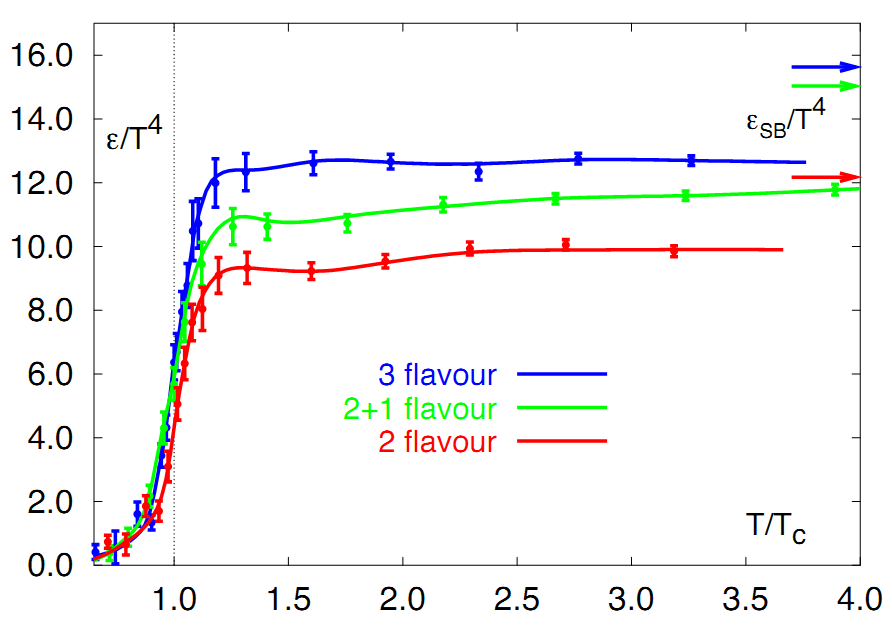
\includegraphics[keepaspectratio,width=0.6\textwidth]{introduction/lQCD_PhaseTransistion.png}
\figcaption{The evolution of $\varepsilon/T^{4}$ as a function of temperature for 3 different flavor scenarios. The arrows indicate the Stefan-Boltzmann limit for each scenario.}
 \label{lQCD_PT}
\end{figure}

\begin{figure}[htbp]
\centering
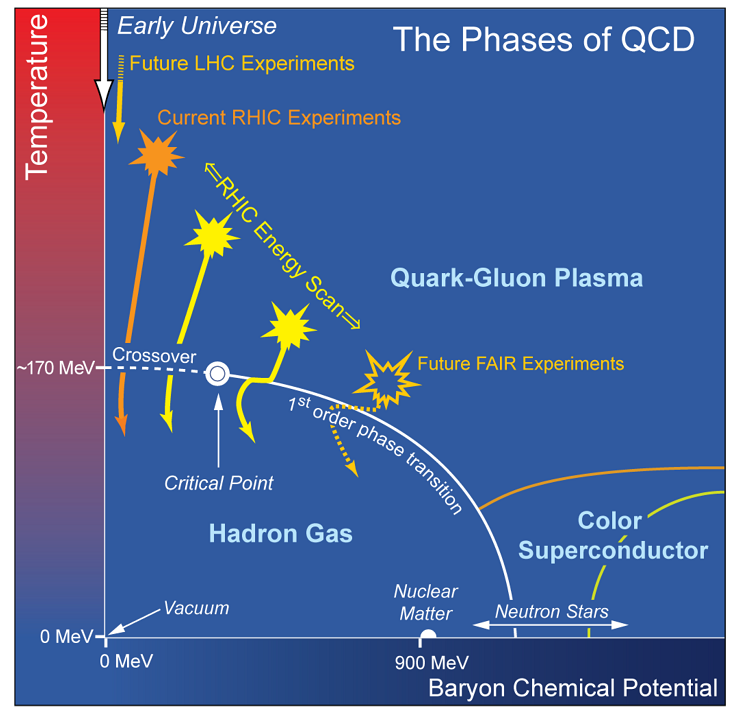
\includegraphics[keepaspectratio,width=0.7\textwidth]{introduction/QCD_phase_diagram.png}
\figcaption{A conjectured QCD phase diagram with boundaries that define various states of QCD matter.}
 \label{QCDpd}
\end{figure}

Figure~\ref{QCDpd} shows a conjectured phase diagram in $T-\mu_{B}$ plane, which describes the phase structure of QCD matter. Lattice QCD calculations predict that the phase transition from hadron gas to the QGP for $T>T_{c}$ at zero baryon chemical potential ($\mu_{B}=$ 0) is expected to be a smooth crossover (white dashed line) instead of a sudden change of energy density. Lattice QCD calculations also predict that there is a first-order phase transition (white solid line) at large $\mu_{B}$, and it is expected to be end in a critical point at finite $\mu_{B}$. The estimation of the location of the critical point~\cite{CriticalPoint} (white dot) is depicted in Fig.~\ref{QCDpd}.

The first RHIC Beam Energy Scan (BES) program was carried out in which data were acquired from Au + Au collisions at $\sqrt{s_{NN}}=$ 62.4, 39, 27, 19.6, 14.5, 11.5, and 7.7 GeV in years 2010, 2011, and 2014~\cite{BESI}. A BES phase \uppercase\expandafter{\romannumeral2} focusing on low collision energies (7.7, 9.1, 11.5, 14.5 and 19.6 GeV) is scheduled to run in years 2019 and 2020~\cite{BESII}. These BES programs can access a broad region of the QCD phase diagram and give us a unique opportunity to search for the QCD critical point and map the first phase boundary.

\subsection{Chiral Symmetry}
The QCD Lagrangian has local $SU(3)_{color}$ gauge symmetry and several global symmetries. For instance,  the $U(1)$ symmetry which entails the baryon number conservation. The QCD Lagrangian has additional symmetries for vanishing quark masses. Compared to momentum transfer of 1 GeV/$c$, the up-, down- and strange-quarks can be treated massless. The Lagrangian is invariant under global vector and axial-vector transformations in $SU(3)$-flavor space
\begin{equation} 
\psi \rightarrow e^{-i\alpha^{i}_{V}\frac{\lambda^{i}}{2}}\psi,  \;\;  \psi \rightarrow e^{-i\alpha^{i}_{A}\frac{\lambda^{i}}{2}\gamma_{5}}\psi
\label{Vec_axiVec_sym}
\end{equation}
When decomposing the quark fields into left and right chirality components, $\psi_{L,R} = \frac{1}{2}(1\mp\gamma_{5})\psi$, the transformations (Eq.~\ref{Vec_axiVec_sym}) translate to 
\begin{equation} 
\psi_{L} \rightarrow e^{-i\alpha^{i}_{L}\frac{\lambda^{i}}{2}}\psi_{L},  \;\;  \psi_{R} \rightarrow \psi_{R}
\label{Left_sym}
\end{equation}
\begin{equation} 
\psi_{R} \rightarrow e^{-i\alpha^{i}_{R}\frac{\lambda^{i}}{2}}\psi_{R},  \;\;  \psi_{L} \rightarrow \psi_{L}
\label{Right_sym}
\end{equation}
which constitutes a global $SU(3)_{L} \times SU(3)_{R}$ chiral symmetry in the limit of vanishing quark masses in flavor space. 

\paragraph{Spontaneous Breaking of Chiral Symmetry}
Symmetry breaking can be distinguished into two types, explicit symmetry breaking and spontaneous symmetry breaking, characterized by whether the equations of motion fail to be invariant or the ground state fails to be invariant. In spontaneous symmetry breaking, the equations of motion of the system are invariant, but the system is not because the ground state is not invariant. We consider a symmetrical upward dome with a though circling the bottom, as shown in Fig.~\ref{MexicanHat}. If a ball is put at the very peak of the dome, the system is symmetrical under center-axial rotation. However, the system is very unstable, the ball will roll down the dome into the trough, a point of the lowest energy, with a small fluctuation on the system. In this scenario, any point in the trough could be the ground state. Obviously, the ground state is not symmetrical, resulting in spontaneous symmetry breaking.

\begin{figure}[htbp]
\centering
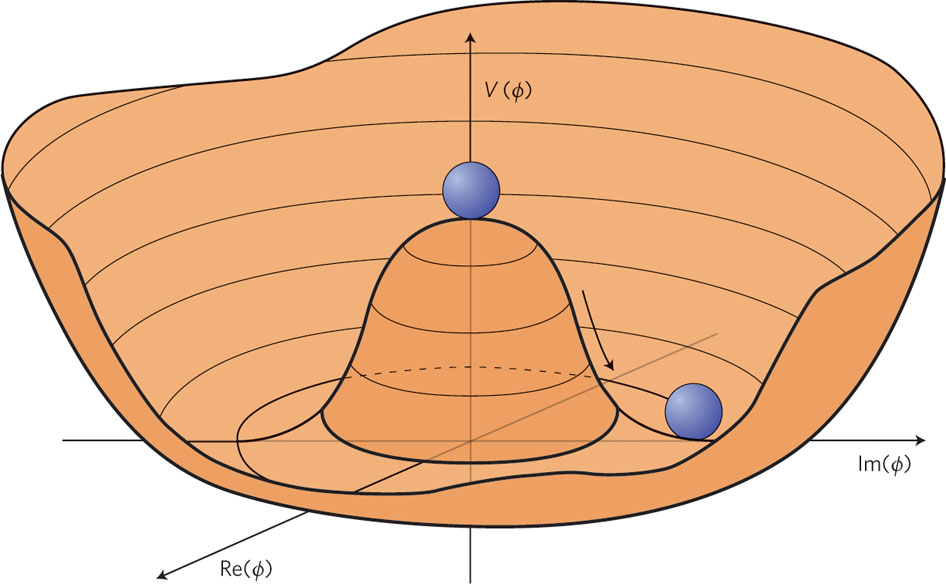
\includegraphics[keepaspectratio,width=0.5\textwidth]{introduction/Mexican_hat.png}
\figcaption{Goldstone's ``Mexican hat'' potential function V versus $\phi$.}
 \label{MexicanHat}
\end{figure}

Chiral symmetry breaking is an example of spontaneous symmetry breaking affecting the chiral symmetry of the strong interactions in particle physics. The vacuum quark condensate can be expressed as the Gell-Mann-Oakes-Renner relation:
\begin{equation} 
m^{2}_{\pi}f^{2}_{\pi} = -2\bar{m}\langle\bar{q}q\rangle
\label{GORrelation}
\end{equation}
where $\bar{m}$ is the average mass of up and down quarks. With $\bar{m}=$ 6 MeV, $m_{\pi}=$ 140 MeV and $f_{\pi}=$ 93.2 MeV, the vacuum condensate is $\langle\bar{q}q\rangle \approx$ (-250 MeV)$^{3}$. A finite quark condensate implies that chiral symmetry is spontaneously broken.  The chiral partner $\rho^{0}$ and $a_{1}(1260)$ have quite different masses ($m_{\rho^{0}}=$ 770 MeV and $m_{a_{1}}=$ 1260 MeV) provides an experimental evidence for spontaneous breaking of chiral symmetry. According to the Goldstone theorem, the spontaneous breaking of chiral symmetry results in the existence of eight massless (very light) Goldstone bosons ($\pi^{\pm}$, $\pi^{0}$, $K^{\pm}$, $K^{0}$, $\bar{K}^{0}$ and $\eta$). 

\paragraph{Restoration of Chiral Symmetry}
In the ultra-relativistic heavy-ion collisions, it is to be expected that the quark and gluon condensates are modified at finite temperature, $T$, and quark chemical potential, $\mu_{q}$. Chiral symmetry restoration can be characterized by the rapid decrease of the quark condensates. Lattice QCD calculations predict a phase transition from hadronic phase to the Quark Gluon Plasma (QGP) phase at high temperature ($T$) and low baryon density or at high baryon density region. The quark condensates are melted in the hot and dense medium, resulting in the restoration of chiral symmetry. The chiral partners will be degenerate when the chiral symmetry restores, which leads to massive medium modifications of hadronic spectral functions as the phase transition approaches. The $\rho$ meson is a unique particle to study the chiral properties of the hot and dense medium, since its life time is much short ($\sim$1.3 fm/$c$) than that of medium ($\sim$10 fm/$c$) created in heavy-ion collisions. Thus $\rho$ meson spectral is very sensitive to the hadronic medium and expected to be significant modified during the system evolution.

\section{Dilepton Production in Heavy-ion Collisions}
\label{dilepton:physics}
Heavy-ion collisions have been pursued for more than several decades for searching and studying the quantum chromodynamics (QCD) matter in the laboratory. Several heavy-ion colliders have been conducted, such as Alternating Gradient Synchrotron (AGS) at BNL, Super Proton Synchrotron (SPS) at CERN, Relativistic Heavy Ion Collider (RHIC) at BNL and Large Hadron Collider (LHC) at CERN. Since year 2000, the RHIC has been operating and providing collisions to its two large experiments STAR and PHENIX, and its two small experiments PHOBOS (decommissioned in 2005) and BRAHMS (decommissioned in 2006). All of these four experiments reported the results from first three years in 2005, and argued that a strongly coupled quark gluon plasma (sQGP) had been established in high-energy heavy-ion collisions~\cite{STARwp,PHENIXwp,PHOBOSwp,BRAHMSwp}. There have been two runs (years 2010 and 2011) at the LHC with Pb + Pb collisions at $\sqrt{s_{NN}}$ = 2.76 TeV, fourteen times higher than RHIC top energy, resulting in hotter, larger size and longer lifetime fire ball. Many of the RHIC findings of the properties of the QGP medium are confirmed by the LHC experiments.

As electromagnetic probes, dileptons play a crucial role in probing hot and dense nuclear matter created in the relativistic heavy-ion collisions. Dileptons are produced in the whole evolution of the created matter and escape with minimum interaction with the strongly interacting medium. Thus, they provide information about the various stages of the system during the evolution. According to different physics interests, the dilepton invariant mass spectrum is typically divided into three ranges: the Low Mass Region (LMR, $M_{ll}<M_{\phi}$), the Intermediate Mass Region (IMR, $M_{\phi}<M_{ll}<M_{J/\psi}$) and the High Mass Region (HMR, $M_{ll}>M_{J/\psi}$), to probe the properties of the created matter throughout its entire evolution.

In the HMR, the dileptons are produced by the initial hard pertubative QCD processes. For instance, the Drell-Yan production ($q\bar{q} \rightarrow \gamma^{*}/Z \rightarrow l^{+}l^{-}$), semi-leptonic decays of correlated heavy quark pairs ($b\bar{b} \rightarrow l^{+}l^{-}$) and heavy quarkonia (J/$\psi$, $\varUpsilon$ etc.). Thus dileptons in the HMR are used to probe the initial stage of the collision~\cite{InitialDilepton}. For instance, the J/$\psi$, $\varUpsilon$ and their excited states are used to study the color screening features of the QGP~\cite{JpsiDeconfinement}.

In the IMR, the dileptons are expected to be directly related to the thermal radiation of the QGP. Theoretical calculations indicate that the QGP thermal dilepton production will become a dominate source in the IMR at top RHIC energy. Thermal dileptons with higher masses originate from earlier stages~\cite{broaden1}. The measurement of the thermal dilepton yields can be used to determine the initial temperature of the QGP medium. However, to measure the dielepton from QGP thermal radiation, the significant contributions from the semi-leptonic decays of correlated open heavy flavor should be measured (e.g.  $c + \overline{c} \rightarrow e + \mu, b \rightarrow e(\mu) + c \rightarrow e + \mu$ ) and subtracted experimentally first.
 
 In the LMR, the dilepton production is dominated by in-medium decay of vector mesons ($\rho$, $\omega$, $\phi$, etc.) and also contributed by long-lived hadron decays ($\pi^{0}$, $\eta$, $\eta^{\prime}$, etc.). Theoretical calculations suggest that the vector meson spectral functions will undergo modifications in a hot and dense hadronic medium, which are considered as a link to chiral symmetry restoration~\cite{broaden0,broaden1,broaden2}. In the vacuum, the chiral symmetry is spontaneously broken, resulting in mass differences between chiral partners (e.g. $\rho$ and $a_{1}$(1260)). In the hot and dense medium, the chiral symmetry is expected to restore, resulting in the degeneration of $\rho$ and $a_{1}(1260)$. However, it is impossible to measure a spectral function for the $a_{1}$(1260) in the heavy-ion collisions. Instead, efforts are devoted to study the modification of vector meson spectral function, and then models are employed to connect the modification function to the chiral symmetry restoration. Two scenarios have been used to describe the in-medium $\rho$ spectral function when chiral symmetry is restored: a dropping mass $\rho$~\cite{dropmass} and a broadened $\rho$~\cite{broaden2}. The dilepton measurements in LMR will map the vector meson production mechanisms, and thus the chiral properties of the medium in heavy-ion collisions. The contributions from long-lived hadron decays can be simulated based on the measured or predicted $p_{T}$ spectra and yields of the involved parent particles, so called hadronic cocktails.

\section{Previous Dilepton Measurements}
For the past decades, lots of dilepton measurements have been carried out in heavy-ion collisions from low to ultrarelativistic energies. For instance, DLS at Bevalac~\cite{DLS:dielectron0,DLS:dielectron1}; HADES at SIS18~\cite{HADES:dielectron0,HADES:dielectron1,HADES:dielectron2,HADES:dielectron3}; HELIOS/3~\cite{HELIOS:dimuon}, NA38/50~\cite{NA38:dimuon,NA50:dimuon}, CERES/NA45 and NA60 at SPS~\cite{CERES:dielectron0,CERES:dielectron1,CERES:dielectron2,CERES:dielectron3,NA60:dimuon0,NA60:dimuon1,NA60:dimuon2}; PHENIX and STAR at RHIC~\cite{PHENIX:dielectron0,PHENIX:dielectron1,STAR:dielectron0,STAR:dielectron1:PRL,STAR:dielectron1,STAR:dielectron2}; ALICE at LHC~\cite{ALICE:dielectron}. In this section, only the results of relevant experiments are briefly discussed. 

\subsection{HADES Experiment}

\begin{figure}[htbp]
\begin{minipage}[htbp]{0.42\linewidth}
\centering
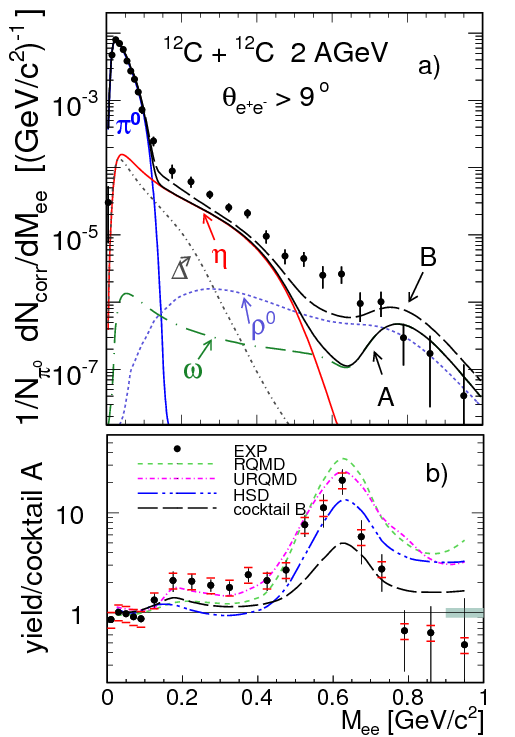
\includegraphics[width=1.0\textwidth]{introduction/HADES_CC_2GeV.png}
\caption{(Top) Dielectron spectrum within HADES acceptance (black dots) together with hadronic cocktail simulations without (Cocktail A, black solid line) and with (Cocktail B, black dashed line) $\Delta(1232)$ and $\rho$ contributions. (Bottom) The ratios of data over cocktail A and cocktail B over cocktail A, together with various model calculations. \label{hades_cc2gev}}
\end{minipage}
\hfill
\begin{minipage}[htbp]{0.56\linewidth}
\centering
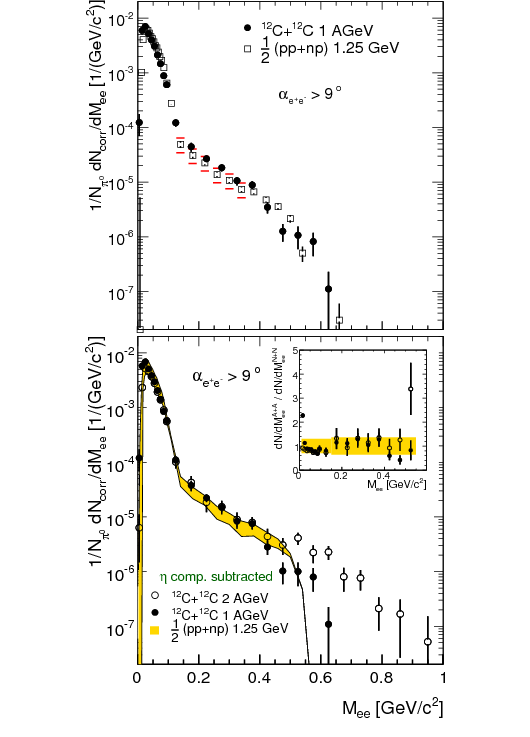
\includegraphics[width=1.0\textwidth]{introduction/HADES_NN_scale.png} 
\caption{(Top) Comparison of the dielectron invariant mass spectrum in $^{12}$C + $^{12}$C collisions at 1 GeV/$u$ (black dots) with an isospin-averaged reference from $p$ + $p$ and $n$ + $p$ collisions (open squares). (Bottom) Comparison of the reference spectrum from elementary collisions with spectra for $^{12}$C + $^{12}$C at 1 (black dots) and 2 GeV/$u$ (open circles). The contribution from $\eta$ Dalitz decay have been subtracted.\label{hades_nnscale}}
\end{minipage}
\end{figure}

\begin{figure}[htbp]
\centering
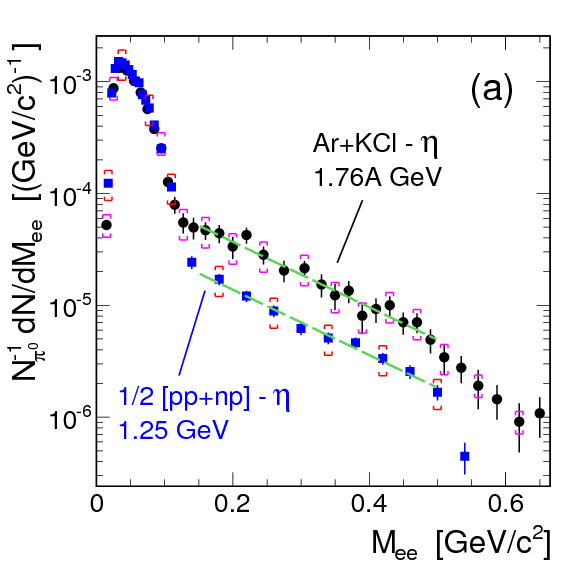
\includegraphics[width=0.48\textwidth]{introduction/HADES_ArKl_0.png}
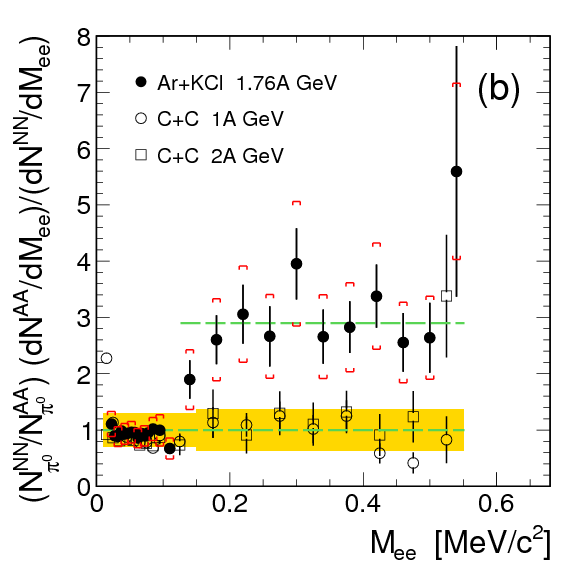
\includegraphics[width=0.48\textwidth]{introduction/HADES_ArKl_1.png}
\figcaption{(Left)  Comparison of the dielectron invariant mass spectrum (subtracted $\eta$ contribution) in Ar + KCl collisions (black dots) with an isospin-averaged reference from $p$ + $p$ and $n$ + $p$ collisions (blue solid squares). (Right) Ratios of $\eta$ contribution subtracted dielectron invariant mass spectra for different collision systems over the reference from $p$ + $p$ and $n$ + $p$ collisions.}
\label{hades_arkcl}
\end{figure}
  
The High-Acceptance DiElectron Spectrometer (HADES) is a fixed target experiment, operated at GSI, with proton and heavy-ion beams being provided by the synchrotron SIS18. HADES reported the dielectron spectra produced in $^{12}$C + $^{12}$C collisions at incident energies of 1 GeV and 2 GeV per nucleon~\cite{HADES:dielectron0,HADES:dielectron1}, and the efficiency-corrected dielectron spectrum within HADES accepctance of 2 A GeV is shown in Fig.~\ref{hades_cc2gev}. The measured dielectron continuum is consistent with the hadronic sources (cocktail) in $\pi^{0}$ region ($M_{ee}<$ 0.15 GeV/$c^{2}$), but a strong excess with respect to cocktail is observed in $M_{ee}>$ 0.15 GeV/$c^{2}$ at both energies. Various transport model calculations are employed, but no one can fully describe the excess. Moreover, the measurements of the excess yields (0.15 $<M_{ee}<$ 0.5 GeV/$c^{2}$) between 1 and 2 A GeV demonstrate that the excess scaled with bombarding energy like pion production, rather than like the production of the much heavier η meson. 
 
HADES also performed the dielectron measurements in elementary $p$ + $p$ and $d$ + $p$ (selecting quasi-free $n$ + $p$ reactions) at incident energy of 1.25 GeV per nucleon~\cite{HADES:dielectron2}. The yield of electron pairs with $M_{ee}>$ 0.15 GeV/$c^{2}$ in quasi-free $n$ + $p$ collisions is about an order of magnitude larger than that in $p$ + $p$ collisions (isospin dependence). Moreover, the excess spectra observed in $^{12}$C + $^{12}$C collisions in 0.15 $<M_{ee}<$ 0.5 GeV/$c^{2}$ at 1 and 2 GeV/$u$ can be described by a superposition of elementary $p$ + $p$ and $n$ + $p$ collisions, as shown in Fig.~\ref{hades_nnscale}, leaving little room for additional electron pair sources in such light collision systems. More recently, the measurements of the dielectron production in Ar + KCl collisions at incident energy of 1.76 GeV per nucleon, observe a significant excess (up to a factor of three) with respect to the $NN$ reference in 0.15 $<M_{ee}<$ 0.5 GeV/$c^{2}$, as shown in Fig.~\ref{hades_arkcl}. This proves that a qualitative change happens in the nature of the excess yield when going to the heavier system, requiring contributions from other sources (e.g. in-medium modifications of the involved hadrons).

\subsection{CERES/NA45 Experiment}
CERES/NA45 is a fixed target experiment dedicated to the measurement of dielectron in the low-mass range from 50 MeV/$c^{2}$ to $\sim$1.5 GeV/$c^{2}$ at the CERN Super Proton Synchrotron (SPS). Particle identification and directional tracking are based on two azimuthally symmetric RICH (ring imaging Cherenkov) detectors, and a detailed description of the CERES/NA45 experiment can be found in~\cite{CERES:experiment}.
 
CERES reported on the measurements of low-mass dielectron spectra in 450 GeV $p$-Be, $p$-Au and 200 A GeV S-Au collisions~\cite{CERES:dielectron0,CERES:dielectron1}. The results are shown in Fig.~\ref{ceres_pASAu}. The measurements of $p$-A can be reproduced within statistical and systematic errors by the hadronic cocktail simulations. However, a significant enhancement with respect to the hadronic cocktail is observed  in $M_{ee}>$ 0.25 GeV/$c^{2}$ in 200 A GeV S-Au collisions. Further dielectron measurements performed in Pb-Au at 40 and 158 A GeV by CERES~\cite{CERES:dielectron2,CERES:dielectron3}, confirm this low-mass region enhancement, as shown in Fig.~\ref{ceres_PbAu}. The $p_{T}^{ee}$ and centrality dependence of the excess spectra have also been studied in Pb-Au collisions at 158 A GeV. The results show the enhancement mostly occurs in low $p_{T}$ region and has a strong centrality dependence. 

\begin{figure}[htbp]
\centering
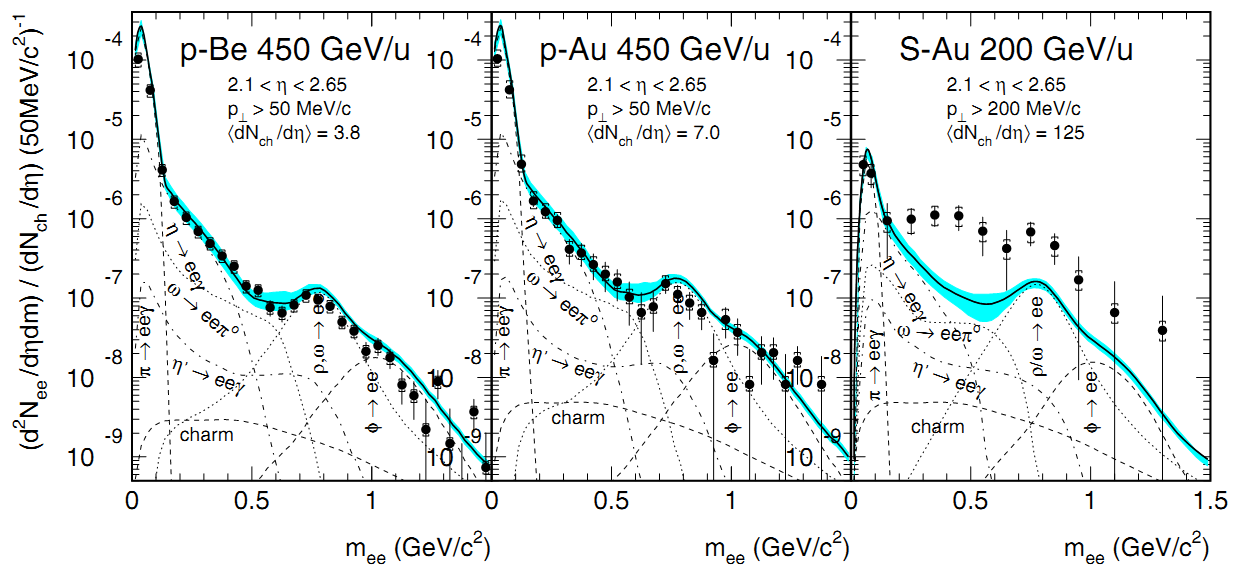
\includegraphics[keepaspectratio,width=1.0\textwidth]{introduction/CERES_pA_SAu.png}
\figcaption{Inclusive dielectron invariant mass spectra (black dots) together with corresponding hadronic cocktails (black solid lines) within CERES acceptance in 450 GeV $p$-Be (Left), $p$-Au (Middle) and 200 A GeV S-Au (Right) collisions.}
 \label{ceres_pASAu}
\end{figure}

\begin{figure}[htbp]
\centering
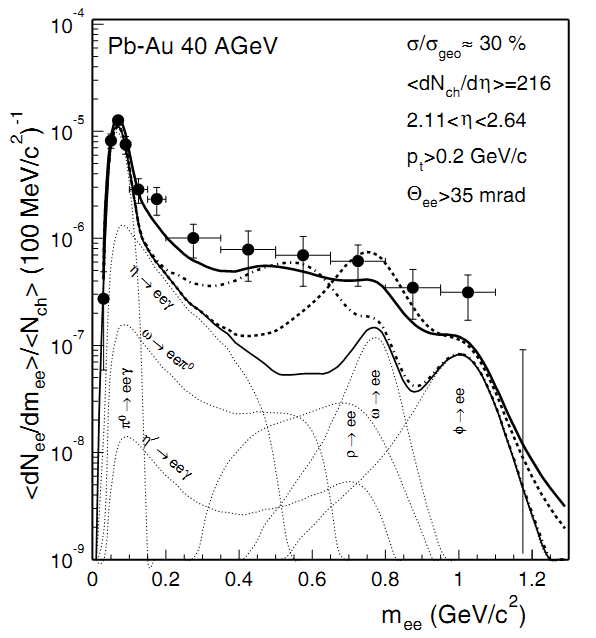
\includegraphics[width=0.468\textwidth]{introduction/CERES_PbAu_40GeV.png}
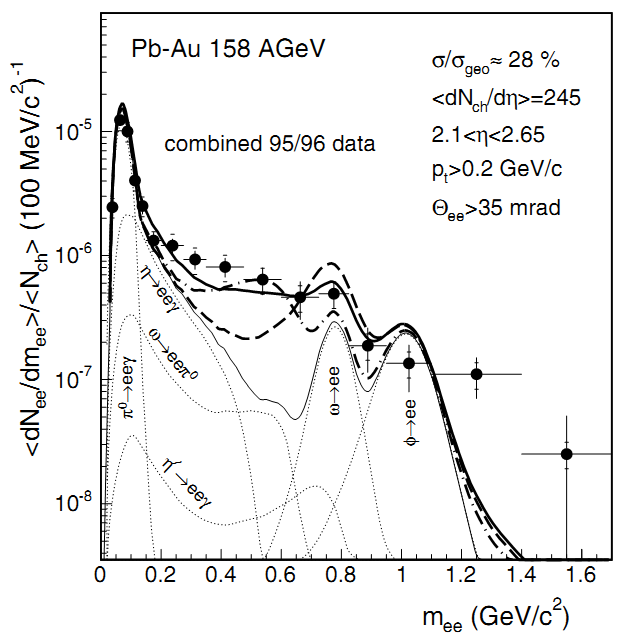
\includegraphics[width=0.48\textwidth]{introduction/CERES_PbAu_158GeV.png}
\figcaption{Comparison of the inclusive mass spectra (black dots) to (i) hadronic cocktails without ρ decay (thin solid line), (ii) model calculations with a vacuum ρ spectral function (thick
dashed line), (iii) with dropping in-medium ρ mass (thick dashed-dotted line), (iv) with a medium-modified ρ spectral function (thick solid line) in Pb-Au collisions at 40 A GeV (Left) and 158 A GeV (Right).}
\label{ceres_PbAu}
\end{figure}

At top SPS energy, the primary candidate for ``thermal radiation'' from the hadronic phase of the fireball is pion annihilation ($\pi^{+}\pi^{-} \rightleftharpoons \rho \rightarrow e^{+}e^{-}$). However, various theoretical models incorporating pion annihilation using vacuum $\rho$ spectral function, fail to describe the data. Thus theoretical calculations incorporating the in-medium modification of $\rho$ meson attempt to reproduce the CERES low-mass region enhancement. Two scenarios are used to describe the in-medium $\rho$ spectrum function: a dropping-mass $\rho$~\cite{dropmass} and a broadened $\rho$~\cite{broaden0}. However, these two scenarios can not be discriminated due to the limited CERES data quality.

\subsection{NA60 Experiment}
NA60 is a fixed target experiment, aiming to study the phase transition from confined hadronic matter to deconfined partonic matter, operated at CERN SPS. NA60 inherits muon spectrometer and zero degree calorimeter previously used in NA38/50~\cite{NA60:dimuon2}. More importantly, a novel radiation-hard silicon pixel vertex tracker with high granularity and high readout speed, placed inside a 2.5 T dipole magnet, is installed the downstream of the targets. Combining the vertex tracker and muon spectrometer, the dimuon mass resolution is significantly improved and the combinatorial background due to $\pi/K$ decays is significantly reduced. Furthermore, the muon offset with respect to the primary interaction vertex can be measured which is essential to distinguish the prompt (Drell-Yan and thermal radiation etc.) and off-vertex (correlated open charm decays) dimuon pairs. The schematic view of the NA60 experiment is shown in Fig.~\ref{NA60experiment}.

\begin{figure}[htbp]
\centering
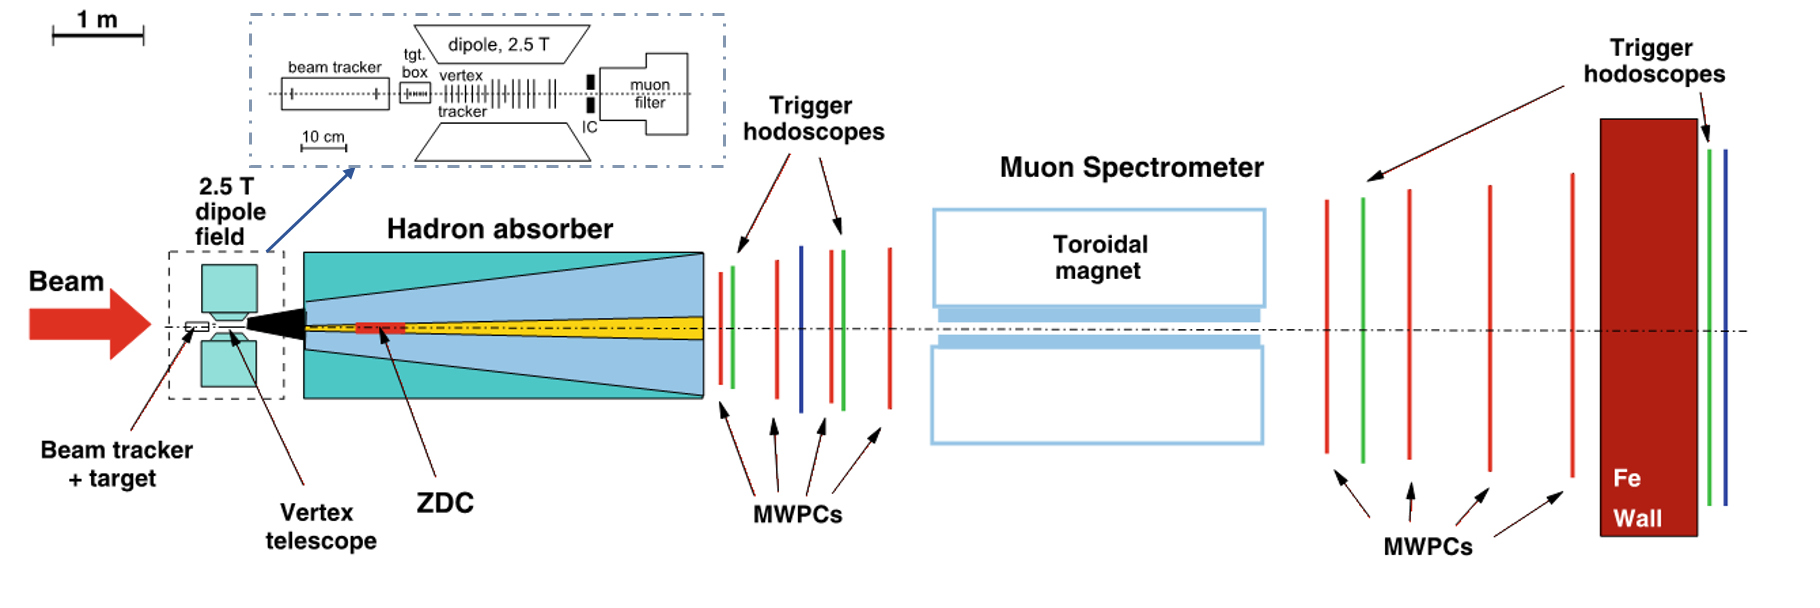
\includegraphics[keepaspectratio,width=1.0\textwidth]{introduction/NA60_experiment.png}
\figcaption{Schematic view of the NA60 experiment.}
 \label{NA60experiment}
\end{figure}

A systematic study of the low mass dimuon spectrum ($M_{\mu\mu}<$ 1.4 GeV/$c^{2}$) has been performed by NA60 using the high precision data in In + In collisions at 158 A GeV. In the most peripheral collisions, the dimuon spectrum can be reproduced by the hadronic cocktail (including the vacuum $\rho$)~\cite{NA60:dimuon0}. However, the dimuon spectrum in the central collisions can not described by the hadronic cocktail any more. A significant enhancement with respect to the hadronic cocktail (excluding $\rho$) is observed, and the excess yield has a strong centrality dependence~\cite{NA60:dimuon3}. The left panel of Fig.~\ref{NA60_LMR_excess} shows the centrality-integrated dimuon mass spectra within NA60 acceptance before (red dots) and after (black triangles) subtraction of the hadronic cocktail (excluding $\rho$), and the right panel shows the excess spectrum in semi-central collisions together with various theoretical model calculations. The theoretical model calculation based on vacuum $\rho$ is clearly ruled out, and the dropping mass scenario which reasonably described the CERES data is also ruled out by the much precise NA60 data. The theoretical model calculation incorporating a broadened $\rho$ spectral function, describes the data reasonably well.

\begin{figure}[htbp]
\centering
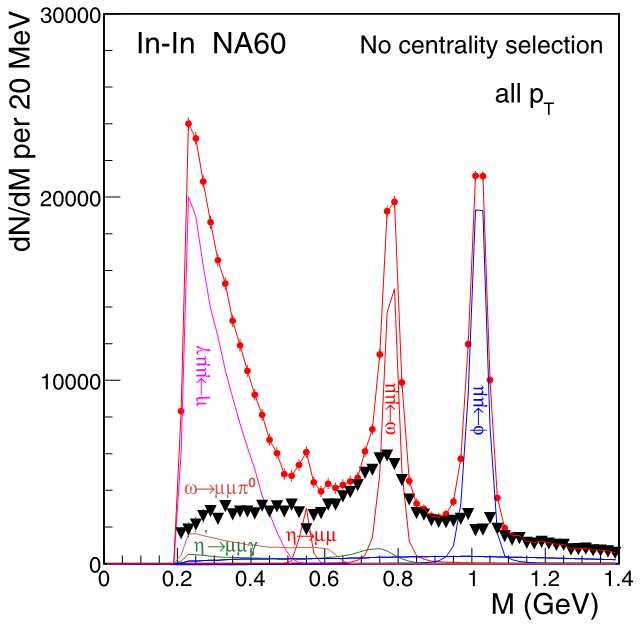
\includegraphics[keepaspectratio,width=0.49\textwidth]{introduction/NA60_LMR_Spec0.png}
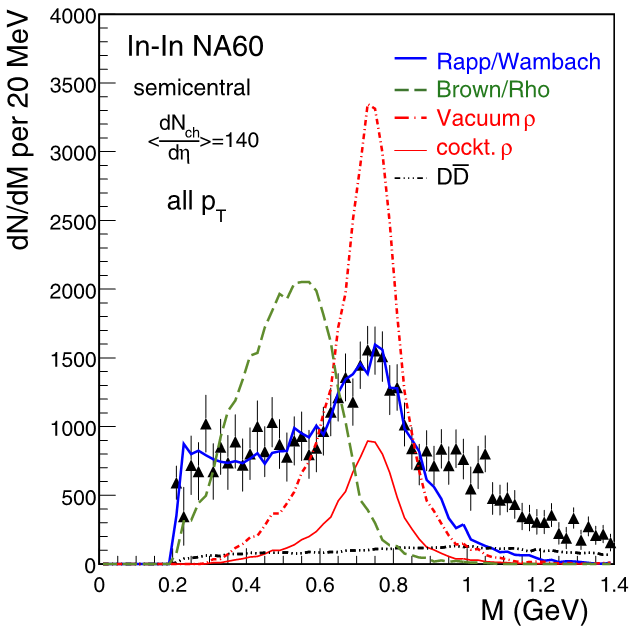
\includegraphics[keepaspectratio,width=0.49\textwidth]{introduction/NA60_LMR_Spec1.png}
\figcaption{(Left) The dimuon spectra within NA60 acceptance before (red dots) and after (black triangles) subtracting the hadronic cocktail (excluding $\rho$). (Right) Excess spectrum within NA60 acceptance in semi-central collisions together with various theoretical model calculations.}
 \label{NA60_LMR_excess}
\end{figure}

For the IMR, thanks to the high position resolution vertex tracker ($\sigma_{x}<$ 10 $\mu$m, $\sigma_{y}<$15 $\mu$m)~\cite{NA60:dimuon2}, the dimuon weighted offset can be measured. The left panel of Fig.~\ref{NA60_IMRdimuon}~\cite{NA60:dimuon2,NA60:dimuon5} shows the dimuon weighted offset distribution for the inclusive dimuon signals in 1.16 $<M_{\mu\mu}<$ 2.56 GeV/$c^{2}$, which is fitted by that of prompt dimuons and open charm decays. The charm cross section is determined by scaling down the NA50 measurements in p-A collisions~\cite{NA50:dimuon}. The fit result shows that the IMR excess is not from the enhancement of open charm decays. After detector acceptance correction, the excess mass spectrum is obtained by subtracting of the open charm and Drell-Yan contributions. The IMR excess mass spectrum drops off much more steeply with mass than that of Drell-Yan pairs while the shape of excess mass spectrum is pretty similar with that of open charms, as shown in the right panel of Fig.~\ref{NA60_IMRdimuon}. Moreover, the excess $p_{T}$ spectra of the three sub mass regions in IMR and ratio of excess over Drell-Yan as a function of $p_{T}^{\mu\mu}$ are also measured, which show the excess in IMR is also not from the enhancement of Drell-Yan process. Strikingly, after removal of the contributions of the correlated open charm (LMR and IMR) and Drell-Yan (only for IMR), the inverse slope parameters ($T_{eff}$) of acceptance-corrected excess $m_{T}$-spectra as a function of  dimuon invariant mass is also measured, as shown in Fig.~\ref{NA60_Teff}. The $T_{eff}$ shows a monotonically rise with mass from dimuon threshold to the nominal pole of $\rho$ meson, and then following a sudden decline by about 50 MeV down to the IMR values. The initial rise is consistent with the expectation for radial flow of an in-medium hadron-like source decaying into dimuon pairs. The sudden decline suggests a transition to a different source, for instance, partonic source argued by NA60 which flow has not yet built up~\cite{NA60:dimuon1,NA60:dimuon2,NA60:dimuon3}.

\begin{figure}[htbp]
\centering
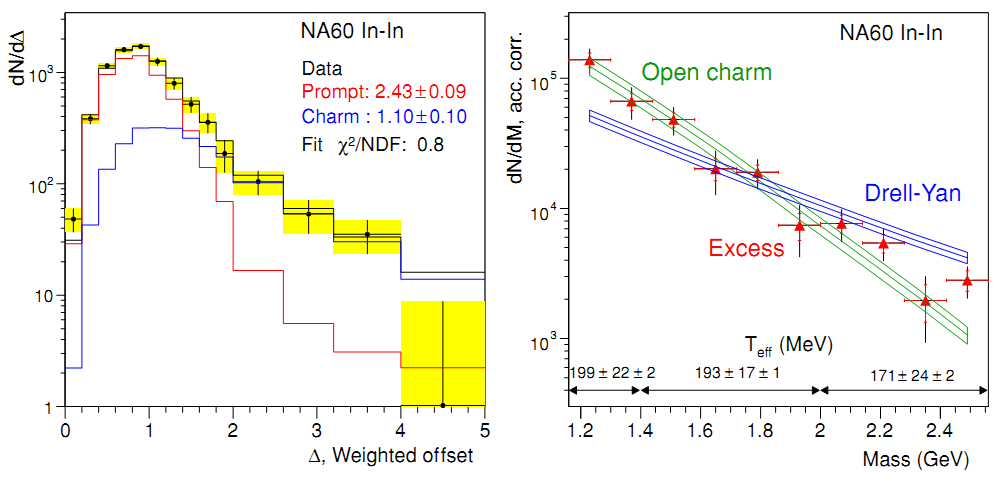
\includegraphics[keepaspectratio,width=1.0\textwidth]{introduction/NA60_dimuon_IMR.png}
\figcaption{(Left) The dimuon weighted offset distribution for the inclusive dimuon signals in 1.16 $<M_{\mu\mu}<$ 2.56 GeV/$c^{2}$ and the comparison with the sum of prompt dimuons and open charm decays. (Right) The detector acceptance corrected mass spectra of all three contributions (excess, Drell-Yan, open charm decays).}
 \label{NA60_IMRdimuon}
\end{figure}

\begin{figure}[htbp]
\centering
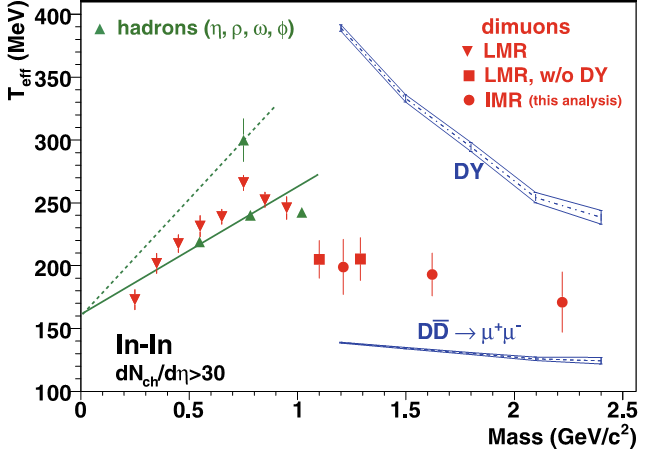
\includegraphics[keepaspectratio,width=0.6\textwidth]{introduction/NA60_InverseSlope.png}
\figcaption{Inverse slope parameter $T_{eff}$ of excess $m_{T}$-spectra as a function of dimuon invariant mass.}
 \label{NA60_Teff}
\end{figure}

\subsection{PHENIX Experiment}
The Pioneering High Energy Nuclear Interaction eXperiment (PHENIX) is one of two large experiments at RHIC. PHENIX is designed specifically to measure direct probes of the collisions such as electrons, muons, and photons.  A detailed description of the detector can be found in~\cite{PHENIX:overview, PHENIX:HBD}.

PHENIX reported the dielectron measurement within PHENIX acceptance in $p$ + $p$ collisions at $\sqrt{s_{NN}}$ = 200 GeV~\cite{PHENIX:dielectron0}, as shown in Fig.~\ref{PHENIX_pp200Spec}, showing that the data can be reproduced by the electromagnetic decays of neutral mesons. The latest dielecton measurements within PHENIX acceptance in Au + Au collisions at $\sqrt{s_{NN}}$ = 200 GeV~\cite{PHENIX:dielectron0}, as shown in Fig.~\ref{PHENIX_AuAu200Spec}, shows that a significant enhancement with respect to the hadronic cocktail can be observed in the LMR. The enhancement factor in 0.30 $<M_{ee}<$ 0.76 GeV/$c^{2}$ is 2.3 $\pm$ 0.4(stat.) $\pm$ 0.4(sys.) $\pm$ 0.2(model) or 1.7 $\pm$ 0.3(stat.) $\pm$ 0.3(sys.) $\pm$ 0.2(model) when the open heavy flavor contribution is  calculated with PYTHIA or MC@NLO, respectively. The new enhancement factor is consistent with that reported by STAR within uncertainty~\cite{STAR:dielectron1}.

\begin{figure}[htbp]
\begin{minipage}[htbp]{0.49\linewidth}
\centering
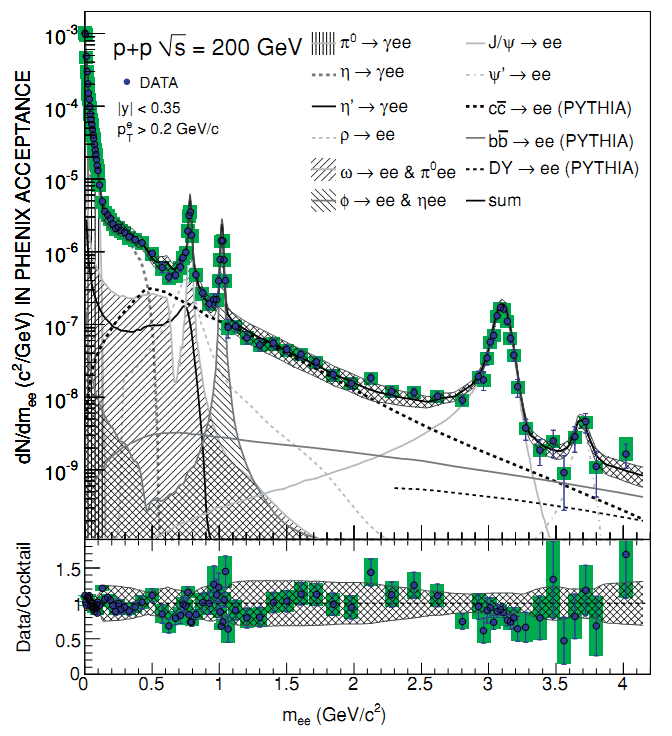
\includegraphics[width=1.0\textwidth]{introduction/PHENIX_pp200.png}
\caption{(Top) Inclusive dielectron invariant mass spectrum together with hadronic cocktail within PHENIX acceptance in $p$ + $p$ collisions at $\sqrt{s_{NN}}$ = 200 GeV. (Bottom) The ratio of data over cocktail as a function of invariant mass. \label{PHENIX_pp200Spec}}
\end{minipage}
\hfill
\begin{minipage}[htbp]{0.49\linewidth}
\centering
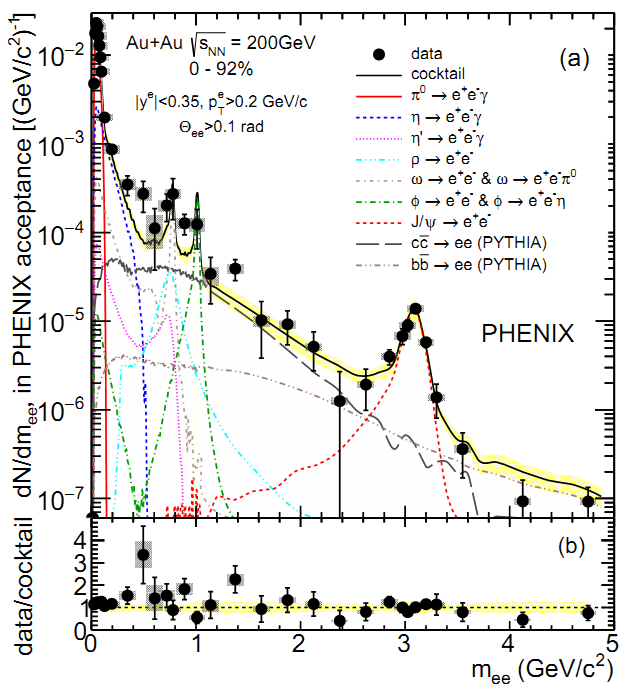
\includegraphics[width=1.0\textwidth]{introduction/PHENIX_AuAu200.png} 
\caption{(Top) Inclusive dielectron invariant mass spectrum together with hadronic cocktail within PHENIX acceptance in Au + Au minimum-bias collisions at $\sqrt{s_{NN}}$ = 200 GeV. (Bottom) The ratio of data over cocktail as a function of invariant mass.\label{PHENIX_AuAu200Spec}}
\end{minipage}
\end{figure}

A theoretical model from Rapp~\cite{broaden0,broaden1,broaden4} incorporating a broadened $\rho$ spectral function and QGP thermal radiation is employed to compare to the PHENIX data, as shown in Fig.~\ref{PHENIX_LMRexcessSpec}. The data can be reasonably described by the model calculation. The integrated excess yield (excess spectrum: data - cocktail) in 0.30 $<M_{ee}<$ 0.76 GeV/$c^{2}$ normalized by number of participants ($N_{part}$) as a function of $N_{part}$ is also measured and shown in Fig.~\ref{PHENIX_LMRexcessYield}. The integrated yield increases faster than $N_{part}$ scaling and is consistent with a expected power-law scaling.

\begin{figure}[htbp]
\begin{minipage}[htbp]{0.49\linewidth}
\centering
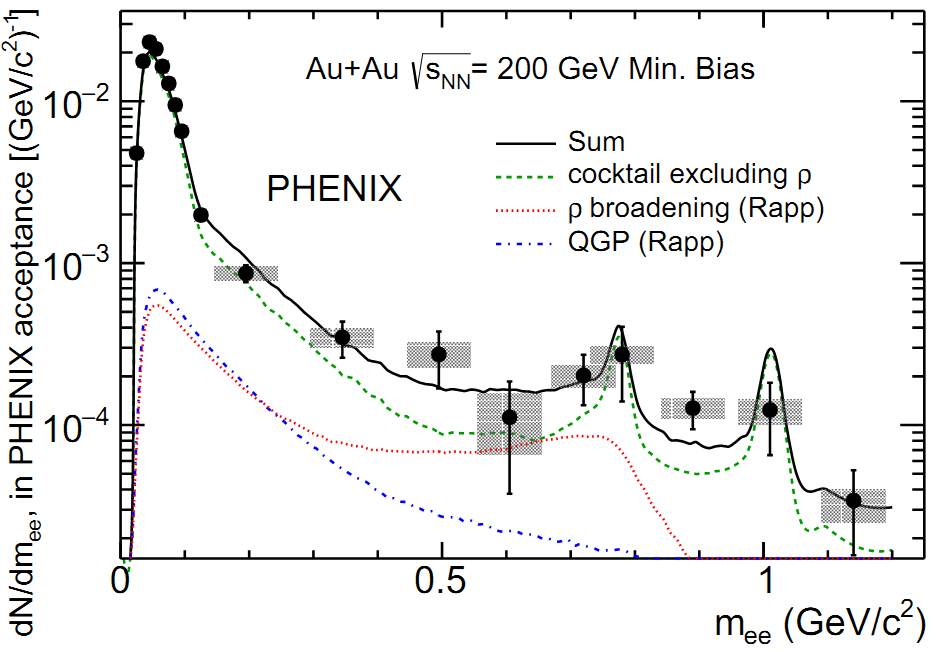
\includegraphics[width=1.0\textwidth]{introduction/PHENIX_LMexcess_Theo.png}
\caption{The minimum-bias invariant mass spectrum together with the model calculations of Rapp. \label{PHENIX_LMRexcessSpec}}
\end{minipage}
\hfill
\begin{minipage}[htbp]{0.49\linewidth}
\centering
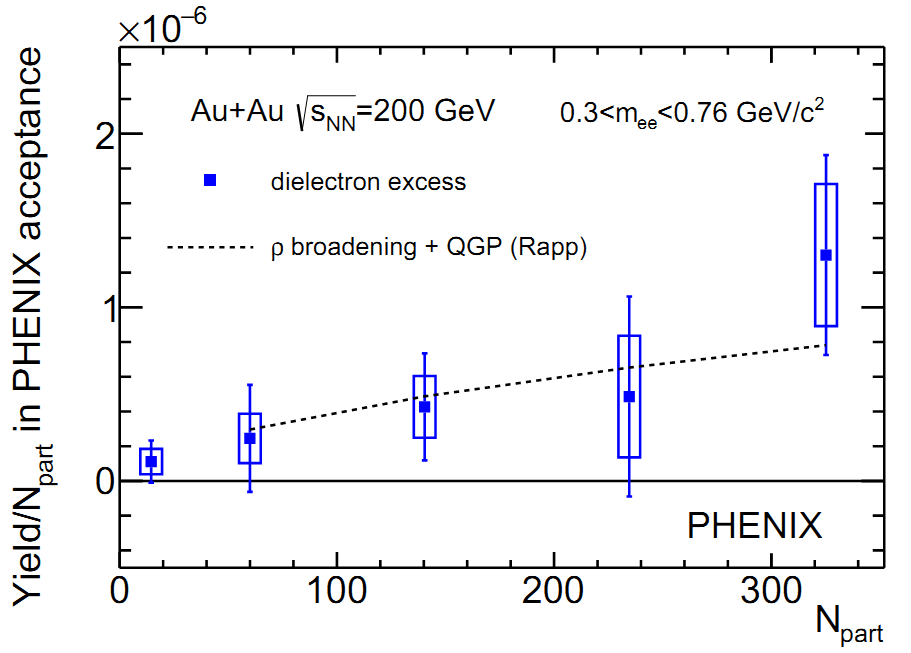
\includegraphics[width=1.0\textwidth]{introduction/PHENIX_LMexcess_Yield.png} 
\caption{Centrality dependence of the dielectron excess (data - cocktail) compared to the thermal radiation from hadronic medium and QGP phase from the model calculations of Rapp.\label{PHENIX_LMRexcessYield}}
\end{minipage}
\end{figure}

\subsection{STAR Experiment}
The Solenoidal Tracker at RHIC (STAR)~\cite{STARdet}, discussed in Sec.~\ref{stardet}, is a general purpose detector located at 6 o'clock of RHIC ring. The dielectron program is enabled with the barrel time-of-flight system upgrade. A (94.6 $\pm$ 1.9)\% overall electron purity can be achieved in Au + Au minimum-bias collisions at $\sqrt{s_{NN}}$ = 200 GeV~\cite{STAR:dielectron1}, combining the Time Projection Chamber (TPC) and Time of Flight (TOF) sub-detectors. 

STAR reported the dielectron measurements within STAR acceptance in $p$ + $p$ collisions at $\sqrt{s_{NN}}$ = 200 GeV using the data taken in year 2009~\cite{STAR:dielectron0}, as shown in Fig.~\ref{STAR_pp200Spec}. Within the uncertainties, the data is consistent with the hadronic cocktail simulation. STAR also reported the dielectron measurements within STAR acceptance in Au + Au collisions at $\sqrt{s_{NN}}$ = 200 GeV using the data taken in years 2010 and 2011~\cite{STAR:dielectron1:PRL,STAR:dielectron1}. The efficiency-corrected dielectron continuum in minimum-bias data and the comparisons with hadronic cocktail simulation and theoretical calculations incorporating broadened $\rho$ spectral functions~\cite{broaden0,broaden1,broaden4,broaden:PHSD0,broaden:PHSD1} (``effective many-body theory model'' and ``microscopic transport dynamic models'') are shown in Fig.~\ref{STAR_AuAu200Spec}. A significant enhancement compare to the hadronic cocktail in LMR ($M_{ee}<$ 1 GeV/$c^{2}$) can be observed, and the enhancement factor in 0.30 $<M_{ee}<$ 0.76 GeV/$c^{2}$ ($\rho$-like region) is 1.76 $\pm$ 0.06 (stat.) $\pm$ 0.26 (sys.) $\pm$ 0.29 (cocktail). The excess spectrum can be reasonably described by theoretical calculations incorporating broadened $\rho$ spectral function and QGP contribution from both Rapp and PHSD. Moreover, the excess in LMR can be consistently observed and described by the model calculations in differential measurements in various $p_{T}$ and centrality bins. The integrated excess yield in $\rho$-like region increases faster than $N_{part}$ scaling and follows a power-law scaling of $N_{part}$ ($\propto$$N_{part}^{1.44 \pm 0.10}$), indicating that the dielctron yield in $\rho$-like region is sensitive to the QCD medium dynamics. 

\begin{figure}[htbp]
\begin{minipage}[htbp]{0.50\linewidth}
\centering
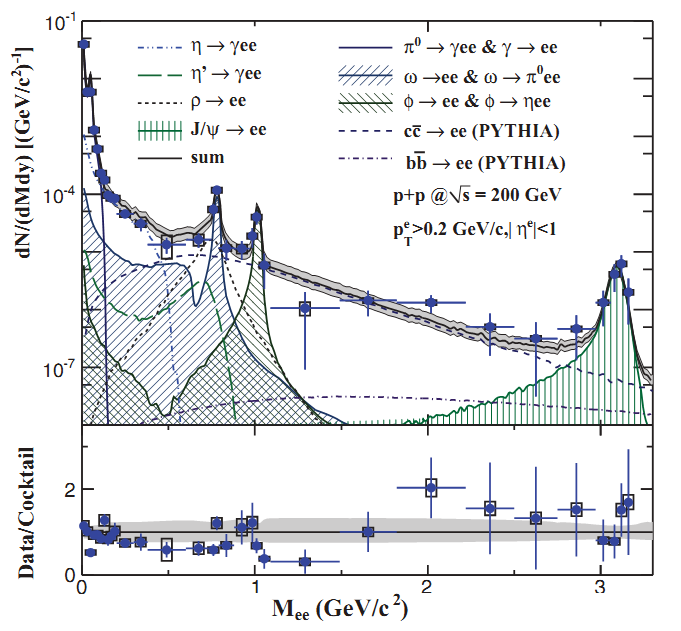
\includegraphics[width=1.0\textwidth]{introduction/STAR_pp200_spec.png}
\caption{(Top) The di-electron continuum after efficiency correction and hadronic cocktail simulation within STAR acceptance in $p$ + $p$ collisions at $\sqrt{s_{NN}}$ = 200 GeV (Bottom) The ratio of data over cocktail as a function of invariant mass. \label{STAR_pp200Spec}}
\end{minipage}
\hfill
\begin{minipage}[htbp]{0.48\linewidth}
\centering
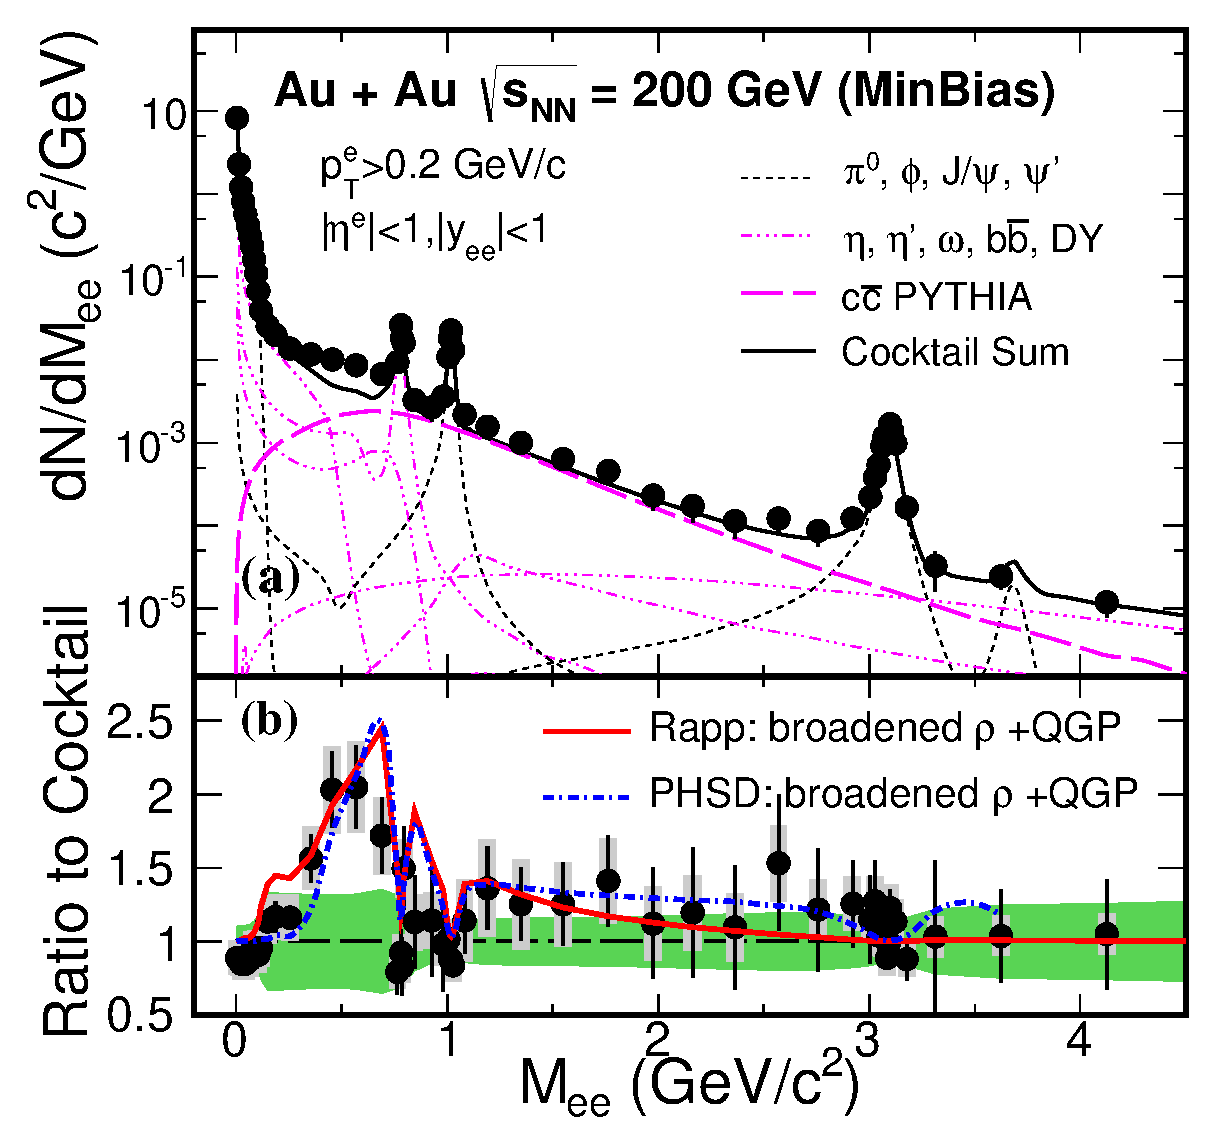
\includegraphics[width=1.0\textwidth]{introduction/STAR_AuAu200_spec.eps} 
\caption{(Top) The invariant mass spectrum from Au + Au minimum-bias collisions at $\sqrt{s_{NN}}$ = 200 GeV compared to a hadronic cocktail simulation. (Bottom) The ratio of data over cocktail as a function of invariant mass and model calculations.\label{STAR_AuAu200Spec}}
\end{minipage}
\end{figure}

\begin{figure}[htbp]
\begin{minipage}[htbp]{0.49\linewidth}
\centering
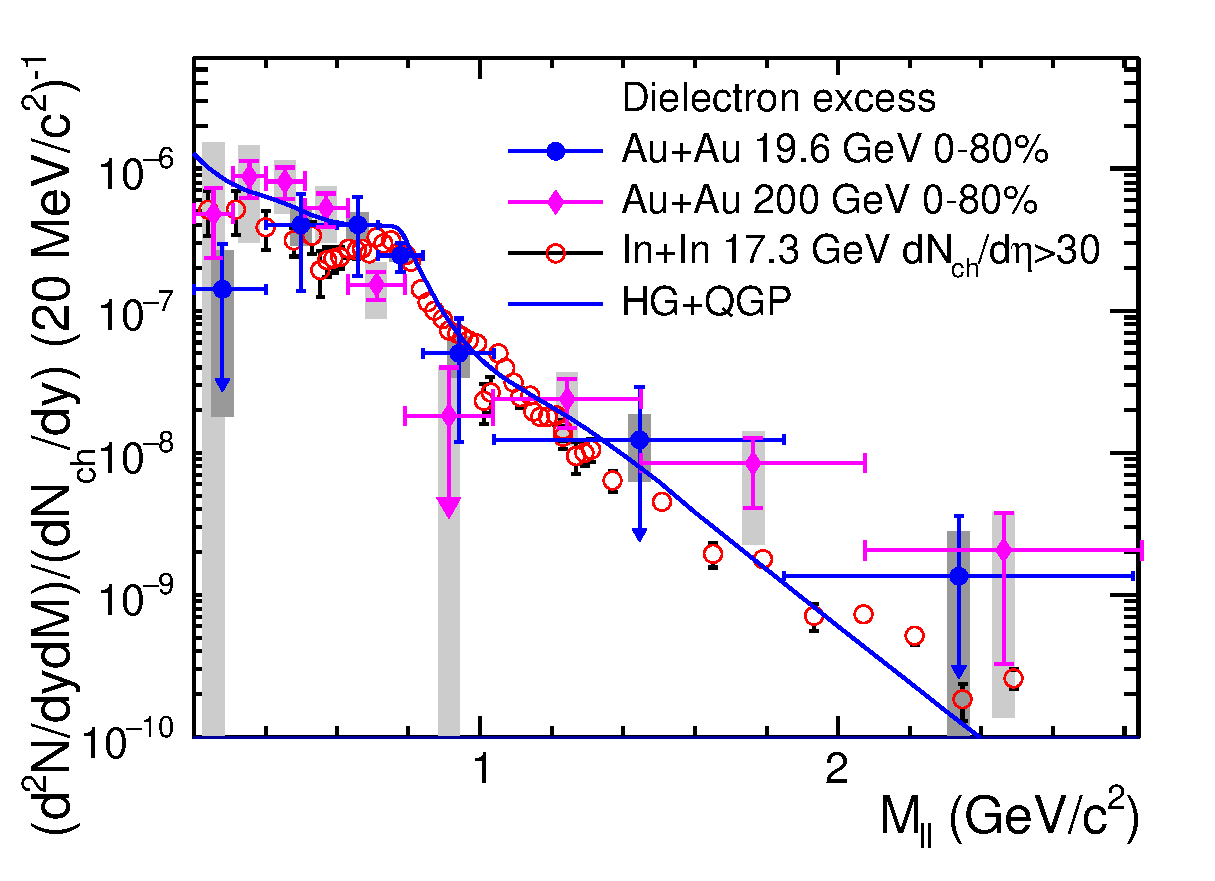
\includegraphics[width=1.0\textwidth]{introduction/STAR_Acc_ExcessSpec.eps}
\caption{The $dN_{ch}/dy$ normalized acceptance-corrected excess dielectron invariant mass spectra in Au + Au collisions at $\sqrt{s_{NN}}$ = 19.6 and 200 GeV, together with that of NA60 in In + In at $\sqrt{s_{NN}}$ = 17.3 GeV. A theoretical model calculation is also added for comparison.\label{STAR_AccExcessSpec}}
\end{minipage}
\hfill
\begin{minipage}[htbp]{0.49\linewidth}
\centering
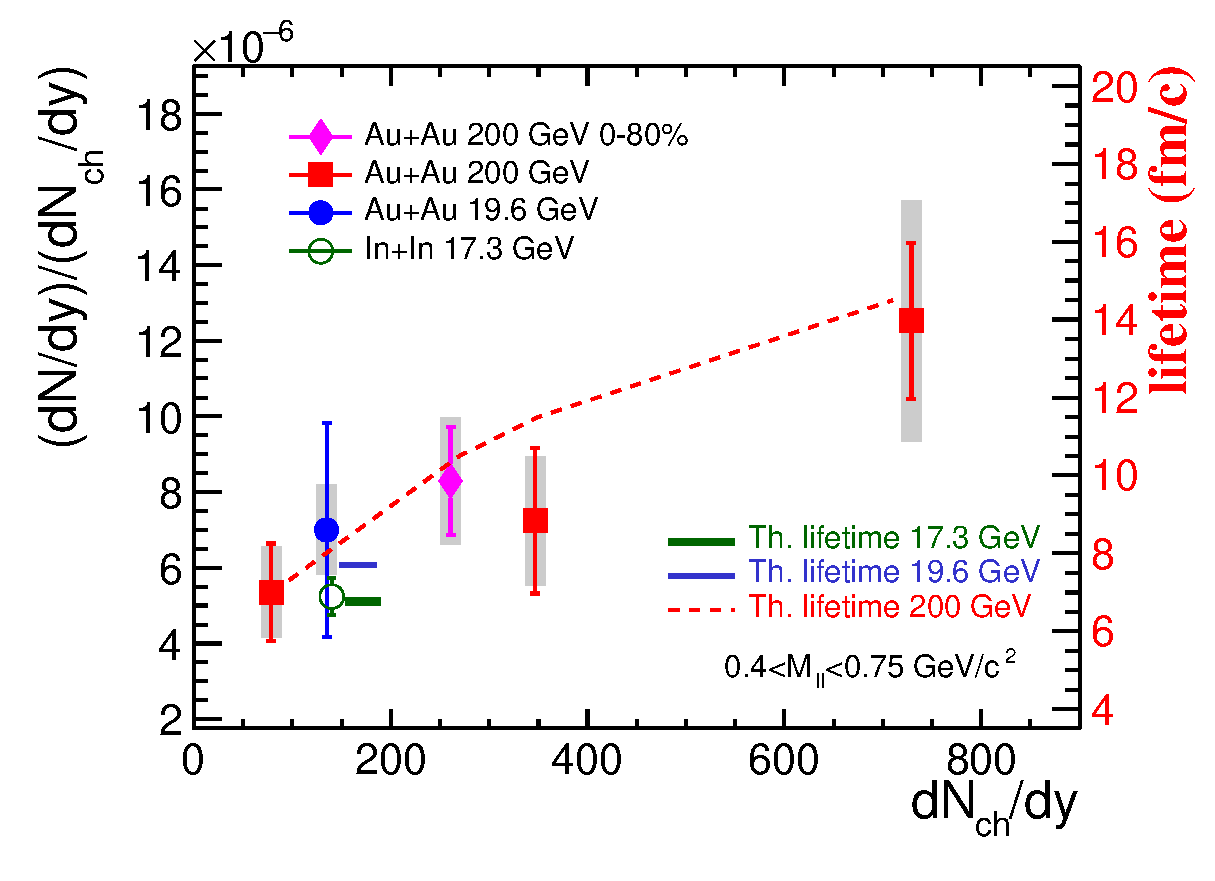
\includegraphics[width=1.0\textwidth]{introduction/STAR_Integrated_ExcessYield.eps} 
\caption{Integrated yields of the normalized dilepton excesses for 0.4 $<M_{ll}<$ 0.75 $GeV/c^{2}$ as a function of $dN_{ch}/dy$ in different collision systems and energies. The theoretical lifetimes are shown as a dashed curve and two horizontal bars.\label{STAR_AccExcessYield}}
\end{minipage}
\end{figure}

To quantitatively study excess dileptons, STAR also measured the acceptance-corrected excess spectra for Au + Au collision at $\sqrt{s_{NN}}$ = 19.6 and 200 GeV, as shown in Fig.~\ref{STAR_AccExcessSpec}. The charged particle density ($dN_{ch}/dy$) normalized excess spectrum in Au + Au collisions at $\sqrt{s_{NN}}$ = 19.6 GeV is similar with that of NA60 in In + In collisions at $\sqrt{s_{NN}}$ = 17.3 GeV within uncertainty in the whole mass region, while the excess at $\sqrt{s_{NN}}$ = 200 GeV is higher than that at $\sqrt{s_{NN}}$ = 17.3 GeV in the LMR and IMR, but within 2$\sigma$ uncertainty. All of the excess spectra can be described by the same model calculation from Rapp incorporating a broadened $\rho$ spectral function and QGP thermal radiation contribution. To quantitatively compare the excess in the LMR, the integrated excess yield in 0.4 $<M_{ee}<$ 0.75 GeV/$c^{2}$ are calculated for Au + Au at $\sqrt{s_{NN}}$ = 19.6 and 200 GeV. The excess yield has a centrality dependence and increases from peripheral to central collisions at $\sqrt{s_{NN}}$ = 200 GeV, and the excess yield in most central Au + Au collisions at 200 GeV is larger than that in lower energies. These measurements might indicate the lifetime of the medium created in Au + Au central collisions at 200 GeV is longer than those in peripheral and/or low-energy collisions, which enhances the dilepton production from thermal radiation.
 
 \begin{figure}[htbp]
\centering
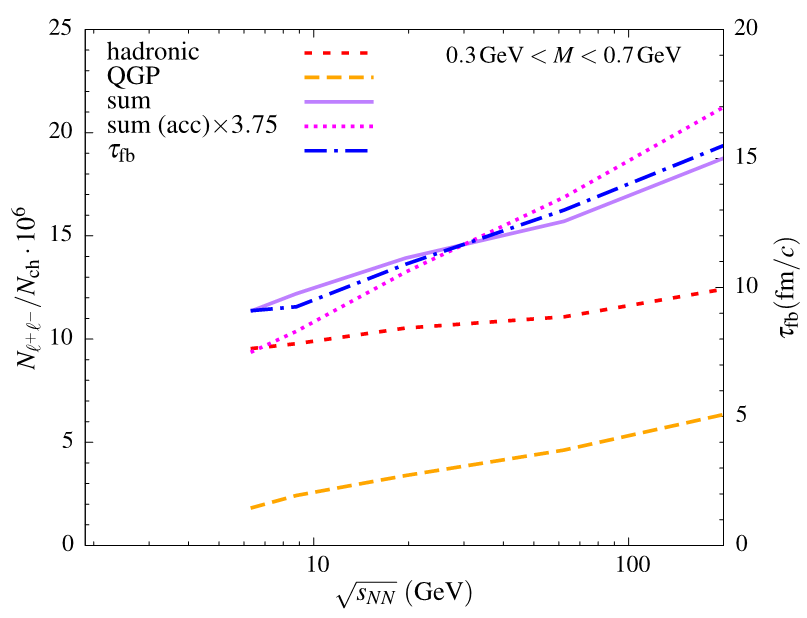
\includegraphics[keepaspectratio,width=0.6\textwidth]{introduction/norExcessYield_vs_energy.png}
\figcaption{Excess spectra in 0–10\% central AA collisions (A$\approx$200), integrated over the mass range $M_{ee}$ = 0.3-0.7 GeV/$c^{2}$, for QGP (dashed line) and in-medium hadronic (short-dashed line) emission and their sum (solid line). The underlying fireball lifetime (dot-dashed line) is given by the right vertical scale.}
 \label{lifetime}
\end{figure}

\section{Advantage of Dielectron Measurements in U + U Collisions at $\sqrt{s_{NN}}$ = 193 GeV}
 The Uranium nucleus is heavier than Gold nucleus, and the energy density created in U + U collisions at $\sqrt{s_{NN}}$ = 193 GeV is expected to be higher by about 20\% than that in Au + Au collisions at $\sqrt{s_{NN}}$ = 200 GeV~\cite{UUEnergyDensity}. The medium created in U + U collisions might have a longer lifetime compared with the Au + Au collisions. Recently, it is found in a model calculation that the charged particle multiplicity ($dN_{ch}/dy$) normalized dilepton excess yield in the low mass region is proportional to the lifetime of the hot, dense medium created in heavy-ion collisions at $\sqrt{s_{NN}}$ = 6 - 200 GeV~\cite{lifetime_cal}, as shown in Fig.~\ref{lifetime}. Thus it would be interesting to measure the normalized dielectron excess yields in U + U collisions and compare with that in Au + Au collisions.